\documentclass[12pt]{article} %set font size and document type
\usepackage{graphicx} % Required for inserting images
\usepackage[useregional]{datetime2} %allow use of \today
\usepackage[margin=1in]{geometry} % set margins
\usepackage{setspace} % allow setting of double and single spacing
\usepackage{hyperref} % creates clickable table of contents
\usepackage{adjustbox} % allows us to rotate images, tables, etc.
\usepackage[table,xcdraw]{xcolor}

\usepackage{enumitem}% http://ctan.org/pkg/enumitem
\setlist[itemize]{nosep, topsep=0pt}


% \usepackage{xcolor}
\usepackage{color, colortbl}

\usepackage{listings}
\newcommand{\lsin}[1]{\lstinline[columns=fullflexible,keepspaces=true,language=Java,basicstyle=\footnotesize\ttfamily]{#1}}

\lstdefinelanguage{Java}{
  columns=fullflexible,keepspaces=true,basicstyle=\scriptsize\ttfamily,
%  basicstyle=\scriptsize\sffamily,
  numbers=left,
  xleftmargin=5.0ex,
  escapechar=@,
  sensitive=true,
  otherkeywords={},
  morekeywords=[1]{int,while,if,public,static,else,return,new,for,return,void},
  keywordstyle={[1]\bfseries\color{blue}},
  numberstyle=\tiny\color{black},
  rulecolor=\color{black},
}

% set up header and footer
\usepackage{titleps,kantlipsum}
\newpagestyle{mypage}{%
  \headrule
  \sethead{\MakeUppercase{\thesection\quad \sectiontitle}}{}{\thesubsection\quad \subsectiontitle}
  \setfoot{}{}{\em{p. \thepage}}
}
\settitlemarks{section,subsection}
\pagestyle{mypage}

% set up title information 
% Students replace project title and their names here
\title{Black Jack
\\
CS482 Software Engineering Team Assignment 2}
\author{Jenna Borowy, Emma Heiser, Chris Plowman, Callie Walker\\
Client: Dr. Nguyen Ho}
\date{\today}

\begin{document}

\maketitle

% creates table of contents
\pagebreak
\tableofcontents
\section*{Abstract}



%[[ text between `[[' and `]]' are comments from me to you and should be
%commented out as you complete various section 

%Put here the \emph{elevator pitch} for your project. 

%IOW a 1-2 paragraph summary of your project
%that includes who the client is and why they need this App.]]

Our project is a Black Jack app for our client Dr. Nguyen Ho. Our client's company is in the market for a profitable Black Jack app that supports online social aspects such as friends, messaging and table creation. 





\pagebreak
% make body of document double spaced for easier feedback writing
\doublespacing 


% include the latex files with the content
\section{Introduction \textbf{TBD}}

[[ No more than one page that provides a short project description and then
sets the stage for the rest of the document. ]]

%This sentence has an example citation~\cite{DBLP:journals/infsof/BinkleyMI22}



\section{Requirements}


%[[
%This section outlines the requirements for the software, primarily via user
%stories. 
%Non-functional requirements are included separately.
%]]


\subsection{User Roles}
\begin{enumerate}
    \item Guest User
    \item Account User
    \item Table Host
    \item Admin
\end{enumerate} 

%[[ Describe the types of users of your App.
%What is their technical expertise, what security level access should they have,
%etc.
%The purpose of this list is to help you ensure you are meeting the clients
%needs in your requirements.
%The names you use here to describe roles should match what you use in your
%user stories and \emph{reflect the clients vocabulary.}

\subsubsection{Guest User}
A Guest User is an user that wishes to play anonymously, or without signing in. A Guest will have limited actions compared to that of other user types, such as an Account User. A Guest will be able to view the tutorial, join games and tables, play games and bet. However, Guests will not be able to add friends, have access to a friends list, they will not keep winnings after they play, they will not be able to make a table or game, and they will not be able to message Admins.

\subsubsection{Account User}
An Account User is a user who is logged in with an account and has the ability to add friends, remove friends, message friends and view a friends list. Additionally, an account user can create tables and games (which for that table, makes them a Host), they keep earnings from games and can view their account history. 

\subsubsection{Table Host}
A Table Host is a specialized Account User. The only time an Account User is promoted to a Table Host is when that user decides to create a table from the lobby. At that time the Account User gains special permissions for that table such as being able to set min/max bet, max number of seats, betting increments etc. Once the Table Host leaves that table, it then goes back to being a regular Account User.

\subsubsection{Admin}
An Admin Account can do everything that every other user type can. Additionally, an Admin can change the credentials and reset the password of an Account User. Admin Accounts also have a special inbox for messages and recommendations from Account Users.

\subsection{Functional Requirement User Stories and Tasks \textbf{[TBD]}}

%[[
%This section lists all your user stories, \emph{organized} by user type and for each user type organized by FIX ME
%[explain here the organization scheme you chose -- by priority? By points? By something else? ].
%]]

%For each user type create a subsubsection of the same format entitled using the
%user type. ]]


%[[ Complete the following for each user story.
%Put a blank line between user stories]]

These are our user stories organized by user type then priority: \\

\textbf{Guest-only Actions:}
\begin{enumerate}

    \item: \textbf{S3: Create Account (2pts)}
    \begin{enumerate}
        \item Priority: High
        \item \textbf{I want} to create an account \textbf{As a} guest  \textbf{So that} I can play with an account.
        \item \textbf{Definition of Done:} I have an account.
        \item \textbf{Depends On:} I don't have an account.
        \item Tasks: S3: Create Account: Make a new account
    \end{enumerate}

    \item: \textbf{S7: Play As Guest (2pts)}
    \begin{enumerate}
        \item Priority: High
        \item \textbf{I want} to play as a guest \textbf{As a} guest user \textbf{So that} I can play anonymously
        \item \textbf{Definition of Done:} I'm playing as a guest.
        \item \textbf{Depends On:} user wants to play anonymously.
        \item Tasks: S7: Play as guest: user wants to play as a guest
    \end{enumerate}
\end{enumerate}

\textbf{Admin-only Actions:}
\begin{enumerate}
    \item: \textbf{S21: Reset Password (2pts)}
    \begin{enumerate}
        \item Priority: High 
        \item \textbf{I want} to reset a user's password \textbf{As an} Admin account \textbf{So that} I can reset a user's password.
        \item \textbf{Definition of Done:} User has a new password.
        \item \textbf{Depends On:} User has an account (S3)
        \item Tasks: S21: Reset Password: reset a user's password
    \end{enumerate}

    \item: \textbf{S22: Modify Profile (2pts)}
    \begin{enumerate}
        \item Priority: Medium
        \item \textbf{I want} to edit a user's profile \textbf{As an} Admin account \textbf{So that} I can update a profile
        \item \textbf{Definition of Done:} User's profile is updated.
        \item \textbf{Depends On:} User has an account (S3)
        \item Tasks: S22: Modify Profile: Admin edits a user's profile.
    \end{enumerate}
\end{enumerate}

\textbf{Account-User-Only Actions}
\begin{enumerate}
    \item: \textbf{S1: Login (2pts)}
    \begin{enumerate}
        \item Priority: High 
        \item \textbf{I want} to login to my account \textbf{As an} Account-User \textbf{So that} I can play with my account.
        \item \textbf{Definition of Done:} User is logged into account.
        \item \textbf{Depends On:} (S3)
        \item Tasks: S1: Login: login to account
    \end{enumerate}

    \item: \textbf{S2: Logout (1pt)}
    \begin{enumerate}
        \item Priority: High 
        \item \textbf{I want} to logout of account \textbf{As an} Account-user \textbf{So that} I can logout of my account.
        \item \textbf{Definition of Done:} User has logged out of account.
        \item \textbf{Depends On:} user is logged in (S1)
        \item Tasks: S2: Logout: logout of account
    \end{enumerate}

    \item: \textbf{S5: Add Friend (1pt)}
    \begin{enumerate}
        \item Priority: High 
        \item \textbf{I want} to add a friend \textbf{As an} Account-user \textbf{So that} I can have that user registered as a friend.
        \item \textbf{Definition of Done:} Friend shows up in list.
        \item \textbf{Depends On:} (S1)
        \item Tasks: S5: Add Friend: Add friend to friends list
    \end{enumerate}

    \item: \textbf{S6: Remove Friend (1pt)}
    \begin{enumerate}
        \item Priority: High 
        \item \textbf{I want} to remove a friend from friends list \textbf{As an} Account-user \textbf{So that} I can remove a friend from my list.
        \item \textbf{Definition of Done:} Friend is no longer in list.
        \item \textbf{Depends On:} User is in friends list (S5)
        \item Tasks: S6: Remove Friend: Remove friend from list
    \end{enumerate}

    \item: \textbf{S4: View Friends List (1pt)}
    \begin{enumerate}
        \item Priority: High 
        \item \textbf{I want} to view my friends list \textbf{As an} Account-user \textbf{So that} I can see my friends list
        \item \textbf{Definition of Done:} I can see my friends list on screen
        \item \textbf{Depends On:} user has friends added (S5)
        \item Tasks: S4: View Friends List: open and view friends list
    \end{enumerate}

    \item: \textbf{S8: Create Table (2pts)}
    \begin{enumerate}
        \item Priority: High 
        \item \textbf{I want} to create a table for blackjack \textbf{As an} Account-user \textbf{So that} I can make a new table for blackjack
        \item \textbf{Definition of Done:} There is a new table in the lobby
        \item \textbf{Depends On:} User is in lobby
        \item Tasks: S8: Create Table: create a new table for blackjack
    \end{enumerate}

    \item: \textbf{S20: Send Message to Friends (2pts)}
    \begin{enumerate}
        \item Priority: Medium
        \item \textbf{I want} to message friends \textbf{As an} Account-user \textbf{So that} I can chat with my friends
        \item \textbf{Definition of Done:} The chat is sent and my friend can see it
        \item \textbf{Depends On:} user has a friend (S5)
        \item Tasks: S20: Send Message to Friend: send a message to friend
    \end{enumerate}

    \item: \textbf{S15: Send Chat (2pts)}
    \begin{enumerate}
        \item Priority: Low
        \item \textbf{I want} to send chat \textbf{As an} Account-user \textbf{So that} I can send a chat to the table.
        \item \textbf{Definition of Done:} The chat is sent to the table.
        \item \textbf{Depends On:} User is at table (S10)
        \item Tasks: S15: Send Chat: user sends chat to table
    \end{enumerate}

    \item: \textbf{S19: Message Admin (2pts)}
    \begin{enumerate}
        \item Priority: Low 
        \item \textbf{I want} to send an admin a message \textbf{As an} Account-user \textbf{So that} I can contact an admin
        \item \textbf{Definition of Done:} The message is sent and the admin can see it
        \item \textbf{Depends On:} user is an account user and logged in (S1,S3)
        \item Tasks: S19: Message Admin: send message to admin
    \end{enumerate}

    \item: \textbf{S16: View Game History (2pts)}
    \begin{enumerate}
        \item Priority: Low
        \item \textbf{I want} to view my game history \textbf{As an} Account-user \textbf{So that} I can see my wins and losses
        \item \textbf{Definition of Done:} I see the number of games I have won and loss.
        \item \textbf{Depends On:} User has played at least 1 game and is in lobby (S26)
        \item Tasks: S16: View Game History: see games won and loss
    \end{enumerate}
    
\end{enumerate}

\textbf{Any-User Actions:}
\begin{enumerate}
    \item: \textbf{S18: View Tutorial (1pt)}
    \begin{enumerate}
        \item Priority: High
        \item \textbf{I want} To see the tutorial \textbf{As} Any user \textbf{So that} I know how to play the game
        \item \textbf{Definition of Done:} user is at the tutorial page
        \item \textbf{Depends On:} user is in lobby
        \item Tasks: S18: View Tutorial: redirected to a page on how to play blackjack
    \end{enumerate}

    \item: \textbf{S17: Request Chips (2pts)}
    \begin{enumerate}
        \item Priority: High
        \item \textbf{I want} to request chips \textbf{As} Any user \textbf{So that} I can get chips when I've ran out 
        \item \textbf{Definition of Done:} I get chips
        \item \textbf{Depends On:} User is out of chips
        \item Tasks: S17: Request Chips: get chips when I've run out 
    \end{enumerate}
    
    \item: \textbf{S10: Join Table (2pts)}
    \begin{enumerate}
        \item Priority: High
        \item \textbf{I want} to join a table \textbf{As} Any user \textbf{So that} I can be in a table for blackjack
        \item \textbf{Definition of Done:} when I am in the blackjack table
        \item \textbf{Depends On:} user is in lobby 
        \item Tasks: S10: Join Table: user joins a blackjack table
    \end{enumerate}

    \item: \textbf{S12: Join Game (2pts)}
    \begin{enumerate}
        \item Priority: High
        \item \textbf{I want} to join a game \textbf{As} Any user \textbf{So that} I can play the next game of blackjack
        \item \textbf{Definition of Done:} user joins the next game of blackjack
        \item \textbf{Depends On:} user is at table (S10)
        \item Tasks: S12: Join Game : join a game of blackjack
    \end{enumerate}

    \item: \textbf{S26: Play Blackjack (3pts)}
    \begin{enumerate}
        \item Priority: High
        \item \textbf{I want} to play blackjack at a table \textbf{As} Any user \textbf{So that} I can play blackjack
        \item \textbf{Definition of Done:} I'm playing blackjack
        \item \textbf{Depends On:} user is at a table (S10)
        \item Tasks: S26: Play Blackjack : play the blackjack game
    \end{enumerate}

     \item: \textbf{S11: Leave Table (2pts)}
    \begin{enumerate}
        \item Priority: Medium
        \item \textbf{I want} to leave the blackjack table \textbf{As} Any user \textbf{So that} I will no longer be at that table
        \item \textbf{Definition of Done:} user is no longer at that table
        \item \textbf{Depends On:} user is at a table (S10)
        \item Tasks: S11: Leave table : user leaves the blackjack table
    \end{enumerate}

    \item: \textbf{S9: View Table info (2pts)}
    \begin{enumerate}
        \item Priority: Medium
        \item \textbf{I want} to view the table info \textbf{As} Any user \textbf{So that} I can see the specific details of a table
        \item \textbf{Definition of Done:} the table's details are shown
        \item \textbf{Depends On:} user is in lobby
        \item Tasks: S9: View Table info: view table's information
    \end{enumerate}

    \item: \textbf{S14: Change Ace value (1pt)}
    \begin{enumerate}
        \item Priority: Medium
        \item \textbf{I want} to change the ace value in my hand \textbf{As} Any user \textbf{So that} My ace can equal 1 or 11
        \item \textbf{Definition of Done:} When the value of my hand is updated correctly
        \item \textbf{Depends On:} user has an ace and is in game (S12,S26)
        \item Tasks: S14: Change Ace Value: make the ace in my hand 1 or 11
    \end{enumerate}
\end{enumerate}

\colorbox{cyan}{\textbf{Technical Tasks}}

\begin{enumerate}
    \item {T1: Migrate from MySQL to Firebase (1pt)}
    \item {T2: Refactor Game Logic (1pt)}
    \item {T3: Documentation Management (1pt)}
    \item {T4: Refactor Jest testing for Firebase (1pt)}
\end{enumerate}

%\begin{enumerate}
    % For each task write the ID, :, then title. Then describe the task.
        %\item Task [[ ID: Title. Description.]]
    %\end{enumerate}


%\item: \textbf{S15: Open Chat (Table) (2pts)}
%    \begin{enumerate}
%        \item Priority: High 
%        \item \textbf{I want} to open the table chat \textbf{As an} Account-user \textbf{So that} I can see the table's chat.
%        \item \textbf{Definition of Done:} The chat is open on my screen.
%        \item \textbf{Depends On:} user is at a table (S10)
%        \item Tasks: S15: Open Chat: user views the table's chat
%    \end{enumerate}
\subsection{Non-Functional Requirements \textbf{[TBD]}}

[[ Complete the following template for each non-functional requirement. 


\textbf{ID: Title}
\begin{enumerate}
    \item Description:
    \item Affects: 
\end{enumerate}

Categorize the non-functional requirements using subsections using as many
categories as your need.
Please put a blank line between requirements.]]


\subsubsection{Category: User Interface}

\subsubsection{Category: Security}

\subsubsection{Category: Performance}

%\subsubsection{add other subsections as needed, or delete irrelevant subsections}

\section{Iterations} 
\subsection{Sprint 1}
\subsubsection{Plan}
In this sprint we aimed to get a simple working version of Blackjack that runs from a GUI. \\

\noindent We added 6 (Main, card, deck, hand, player, and game).java that serves as our business logic for our game. Additionally we added a login screen that allows the user to sign in, create an account, or play as a guest. We have also implemented the base for our backend database that stores our users login info.

\subsubsection{Activities}

\textbf{User Stories Attempted (Beginning of Sprint 1)}

Callie, Chris 
\begin{itemize}
    \item [--] S26 Play Blackjack (3pts) 
    \item [--] S14 Change Ace Value (1pt)
    \item [--] S21 View Tutorial (1pt)
\end{itemize} 
Jenna, Emma
\begin{itemize}
    \item [--] S1 Login (2pts) 
    \item [--] S2 Logout (1pt)
    \item [--] S3 Create Account (2pts)
    \item [--] S7 Play as Guest (2pts)
\end{itemize} 

Total Points Attempted this Sprint: 12\\

\textbf{User stories Accomplished (End of Sprint 1)}
Callie, Chris
\begin{itemize}
    \item [--] S26 Play Blackjack (3pts)
    \item [--] S21 View Tutorial (1pt)
\end{itemize} 
Jenna, Emma
\begin{itemize}
    \item [--] S1 Login (2pts) 
    \item [--] S3 Create Account (2pts)
\end{itemize} 

Total Points Accomplished this Sprint: 8

\begin{table}[!hbt]
\begin{tabular}{|l|l|l|l|}
\hline
\multicolumn{1}{|c|}{\textbf{Name}} & \multicolumn{1}{c|}{\textbf{Speed}} & \multicolumn{1}{c|}{\textbf{Paired Programming}} & \textbf{Individual Cycle (per/hr)} \\ \hline
Callie & 4 & /2 = 2pts & ~35hrs/2pts = 17.5hrs per point   \\ \hline
Chris  & 4 & /2 = 2pts & ~34hrs/2pts = 16hrs per point \\ \hline
Emma   & 4 & /2 = 2pts & ~29hrs/2pts = 14.5hrs per point   \\ \hline
Jenna  & 4 & /2 = 2pts & ~40hrs/2pts = 20hrs per point \\ \hline
\end{tabular}
\end{table}

\subsubsection{Sprint 1 Testing}

Here are the individual testing results for each member/pair:

Chris/Callie:
\begin{figure}[!hbt]
    \centering
    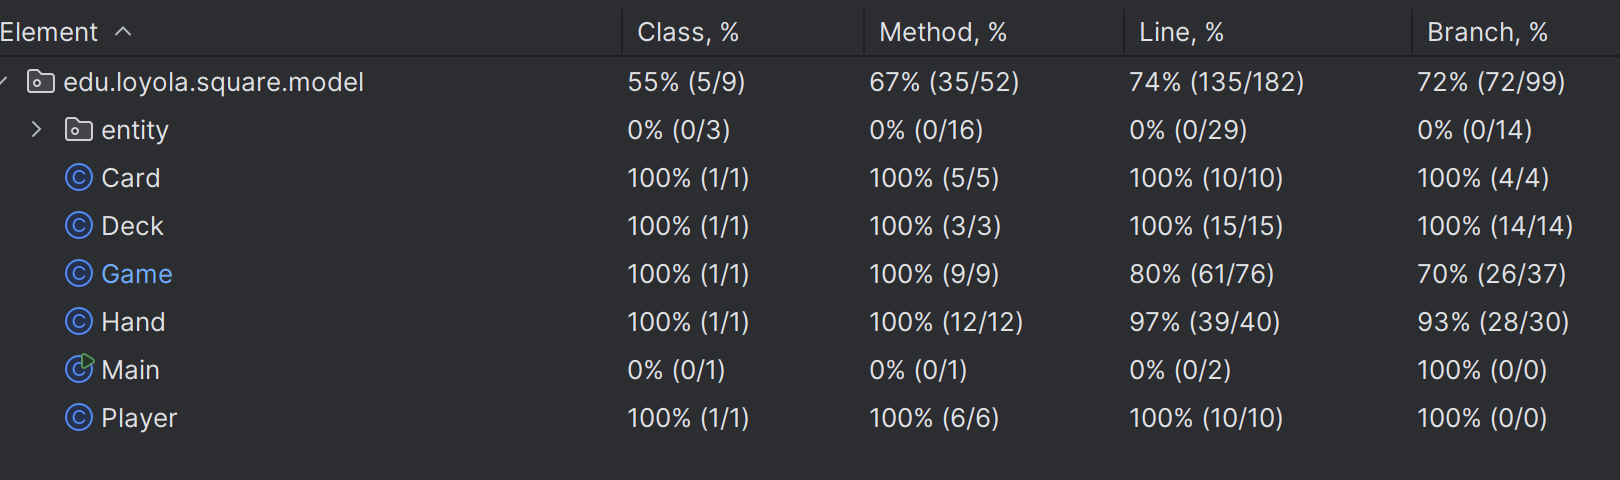
\includegraphics[width=1.0\linewidth]{figures/Coverage report (Model).png}
    \caption{Coverage for Chris/Callie's Code}
    \label{Coverage report}
\end{figure}

Jenna:
\begin{figure}[!hbt]
    \centering
    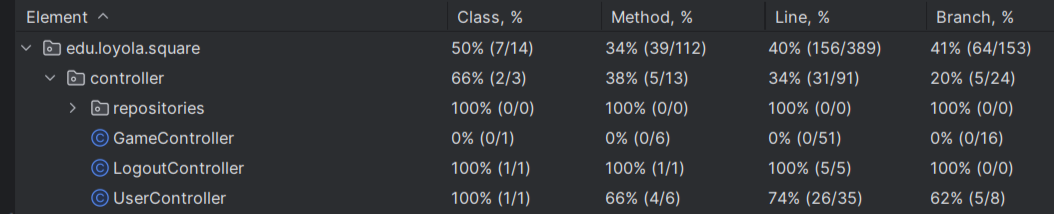
\includegraphics[width=1.0\linewidth]{figures/JennaTest.png}
    \caption{Coverage for Jenna's Code}
    \label{Jenna coverage}
\end{figure}\\


Emma:
\begin{figure}[!hbt]
    \centering
    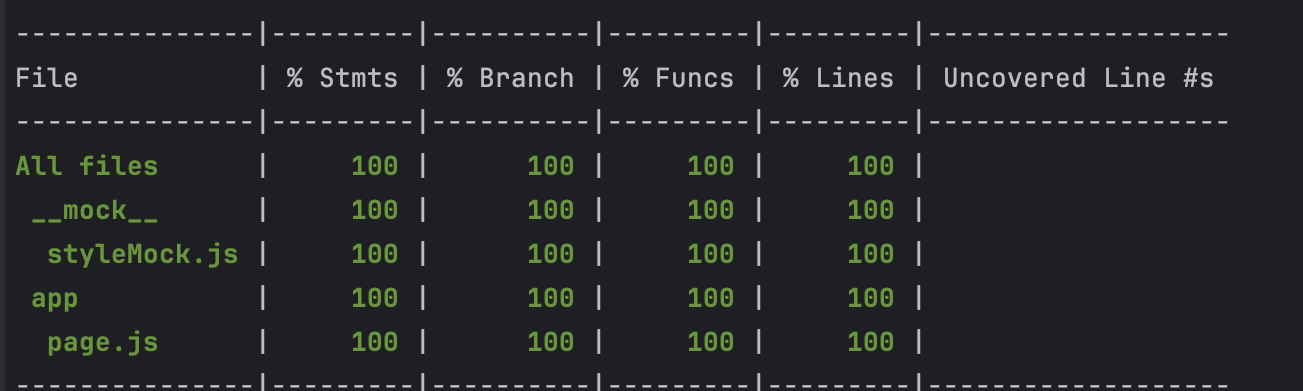
\includegraphics[width=1.0\linewidth]{figures/EmmaTest.png}
    \caption{Coverage for Emma's Code}
    \label{Emma Coverage}
\end{figure}

Callie:
\begin{figure}[!hbt]
    \centering
    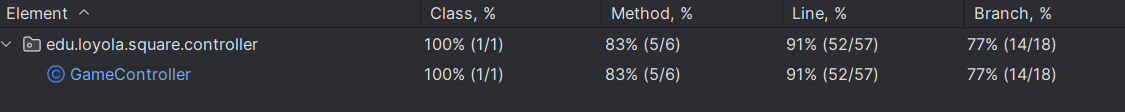
\includegraphics[width=1.0\linewidth]{figures/CallieTest.png}
    \caption{Coverage for Callie's code}
    \label{Callie Coverage}
\end{figure}



\subsubsection{Retrospective}
We realized that integration between model, view and controller can take much more time than anticipated. Additionally, some of our original point values for our user stories might have been underestimated.

%[[ The requirements analysis identifies \textbf{what} your client wants.
%With each iteration describe the \textbf{how}.
%Include user stories attempted, data structures introduced, and any key design
%decisions.

%Copy this layout for each iteration. ]]



\section{Final System Architecture and Design}

\subsection{System Architecture}
Based on our project's requirements and the components involved, we have decided to use the MVC architecture for our project. We believe that the MVC architecture will best let us integrate the major parts of our project (Web UI, functional logic, and database) effectively.

\subsection{Libraries, Modules \& Packages}
So far, we haven't figured out all the libraries and packages we will need for the project. They will be added on a as-needed basis and will be put here.

\subsection{Coding Standards}
\subsubsection{Comments}
Comments (outside of function headers) will always be above the line of code it pertains to, never on the same line. We will aim to keep comments clear, concise and in plain-english.

\subsubsection{Headers}

\begin{itemize}
    \item Function Headers \\
    For functions, we will have consistent headers (in plain-english) including:
    \begin{itemize}
        \item [--] Input: what the function receives as input.
        \item [--] Output: what the function produces.
        \item [--] Purpose: what the function does.
        \item [--] Reliance: function that directly relies on this function, and function that this function directly relies on if any. (for testing purposes)
    \end{itemize}

    \item File Headers \\
    For file headers we will have a brief description of what the file is and what it contains.
\end{itemize}

\subsubsection{Variables}
Following the same standard across all of our code, all variables will be camel case and singular. This guarantees consistency in all variable nomenclature. 

\subsubsection{Database}
For our database, our table names will be Pascal case and singular. The primary keys in our database will be camel case followed by 'ID'. The foreign keys will also be camel case with a descriptor followed by 'FK'.\\

Here is an ER diagram of our database: 

\begin{figure}[hbt!]
    \centering
    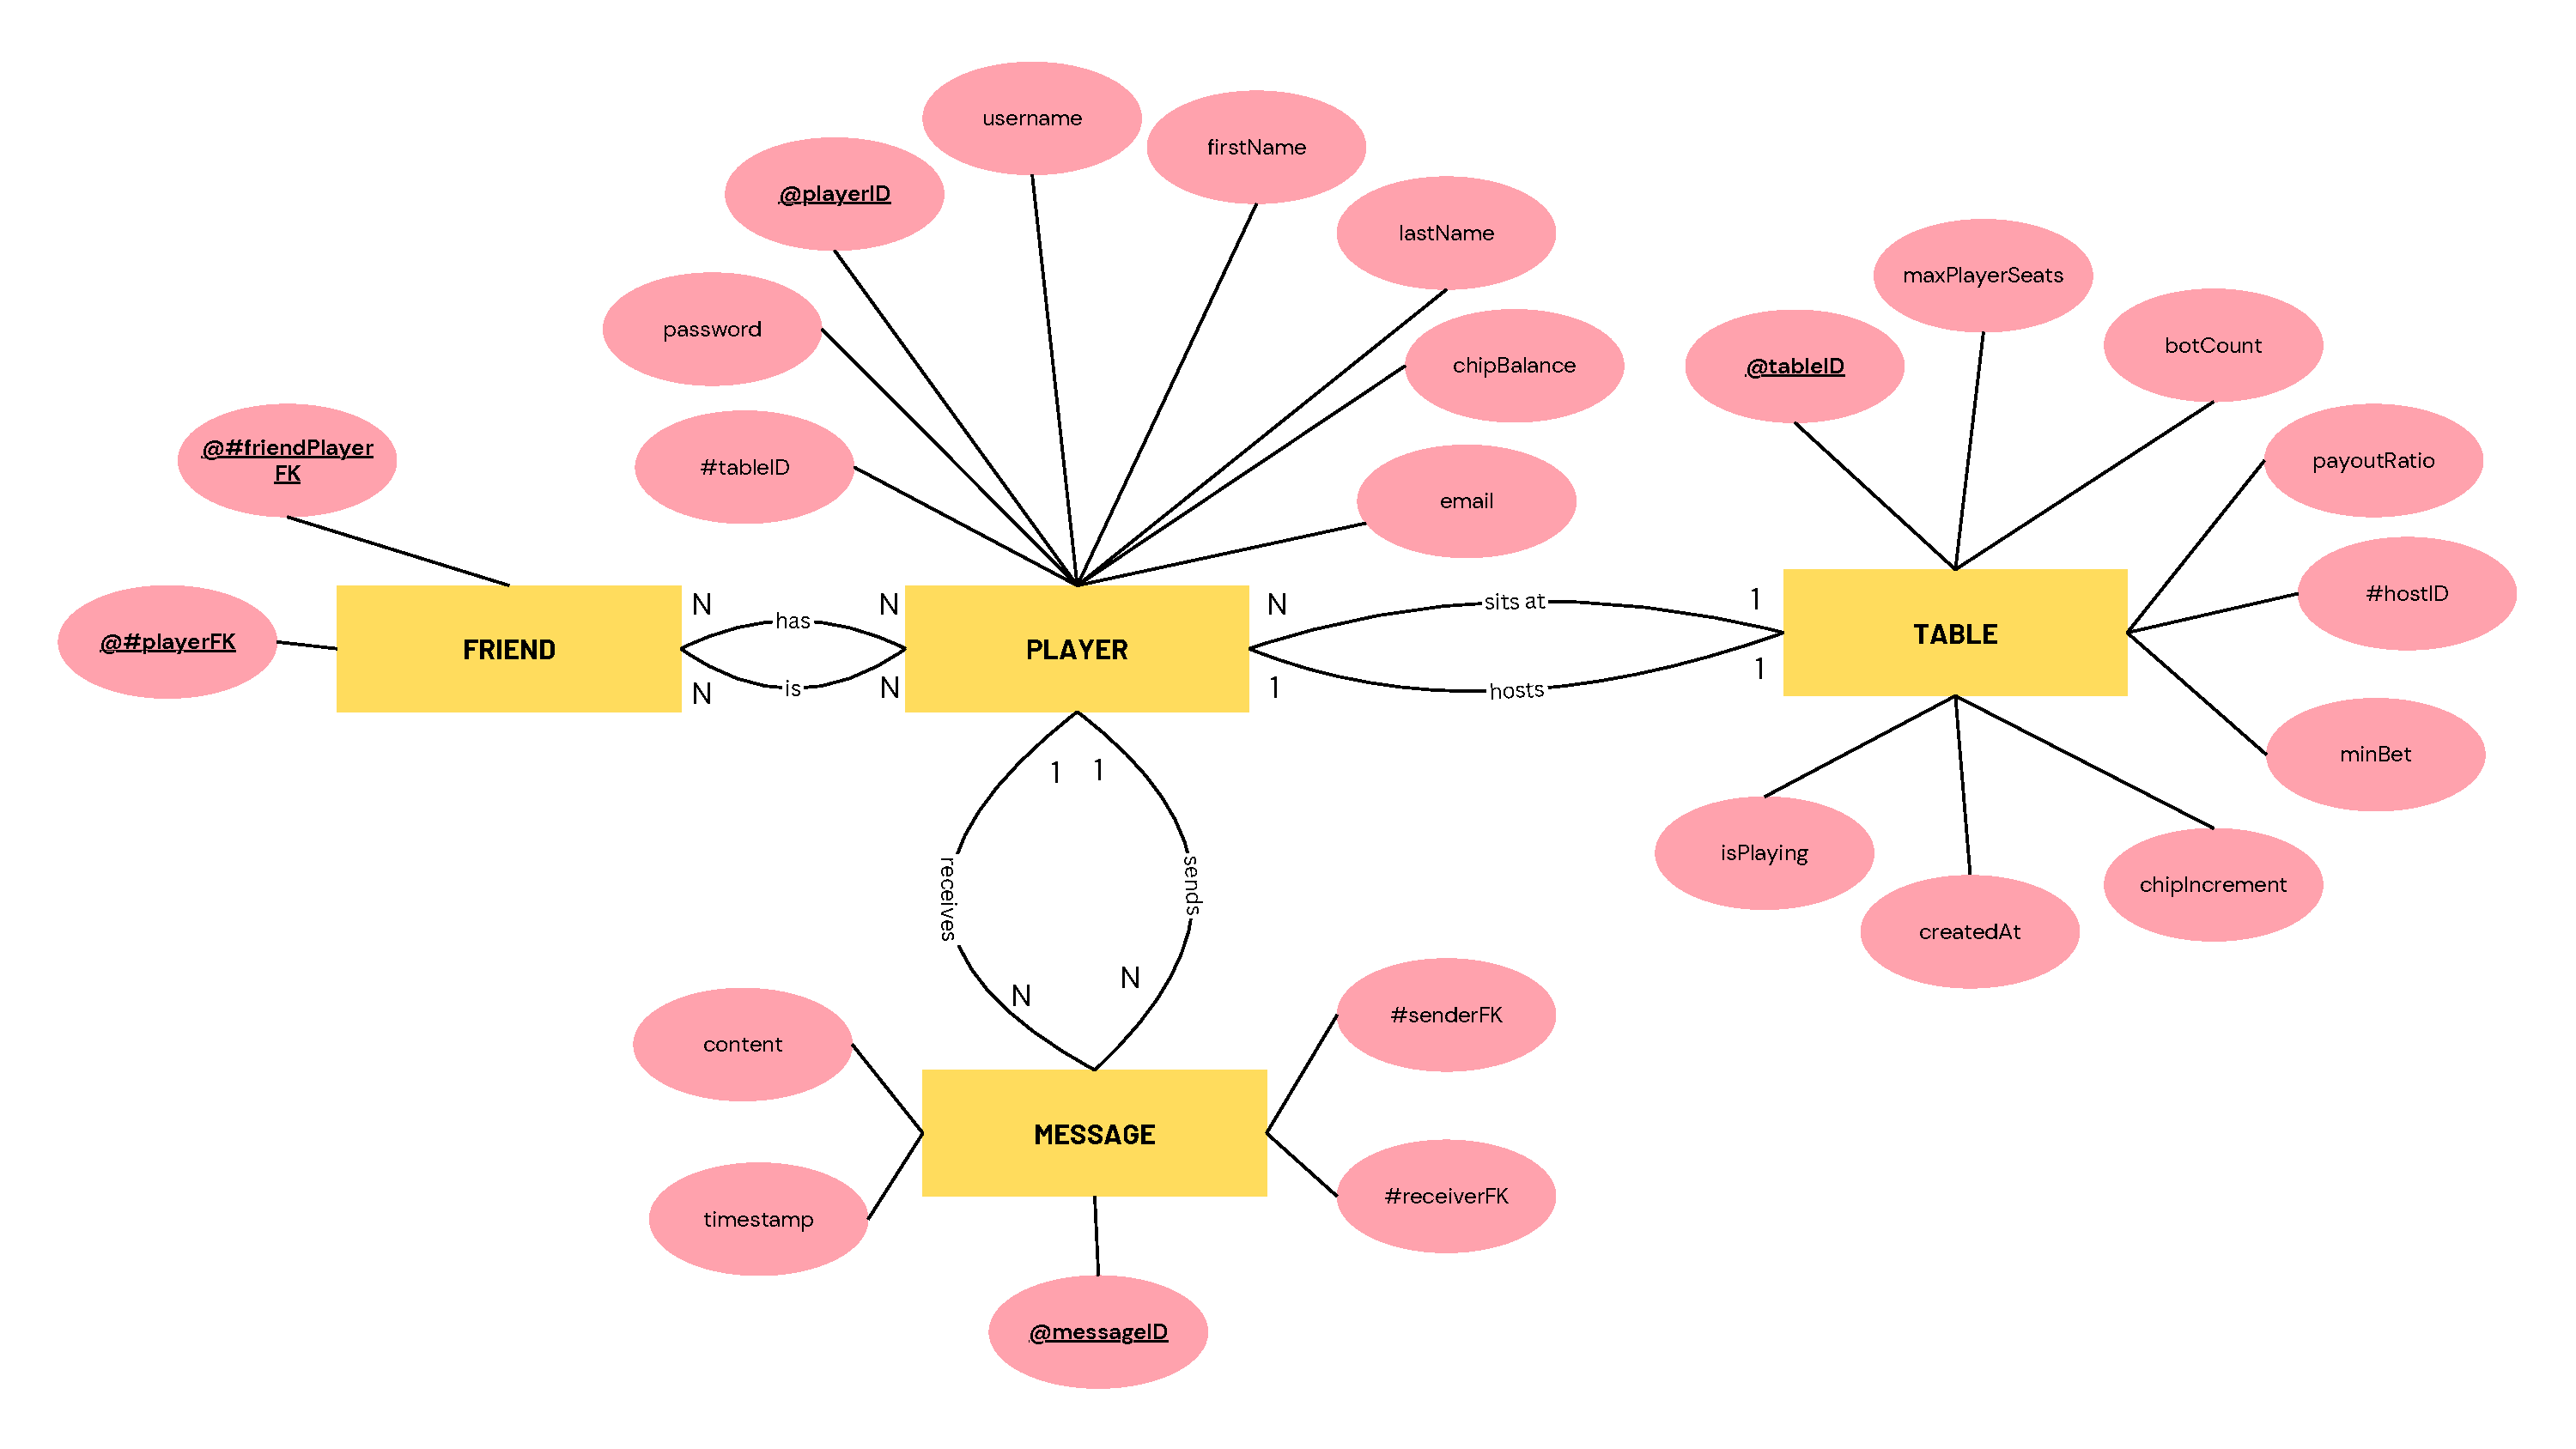
\includegraphics[width=1.0\linewidth]{figures/SE Database ERD.pdf}
    \caption{ERD for our database tables.}
    \label{fig:ERD}
\end{figure} 

\pagebreak

\subsection{Technologies Used}

\subsubsection{Languages}
For the language to run our functional logic we have chose Java as it integrates well with the other languages in our project. For our database components we will be using MySQL along with MySQL community server and MySQL workbench. For our web UI we will be using React along with Next JS for our server.

Here is our UML class diagram that outlines the major classes and relations in our software:  

\begin{figure}[hbt!]
    \centering
    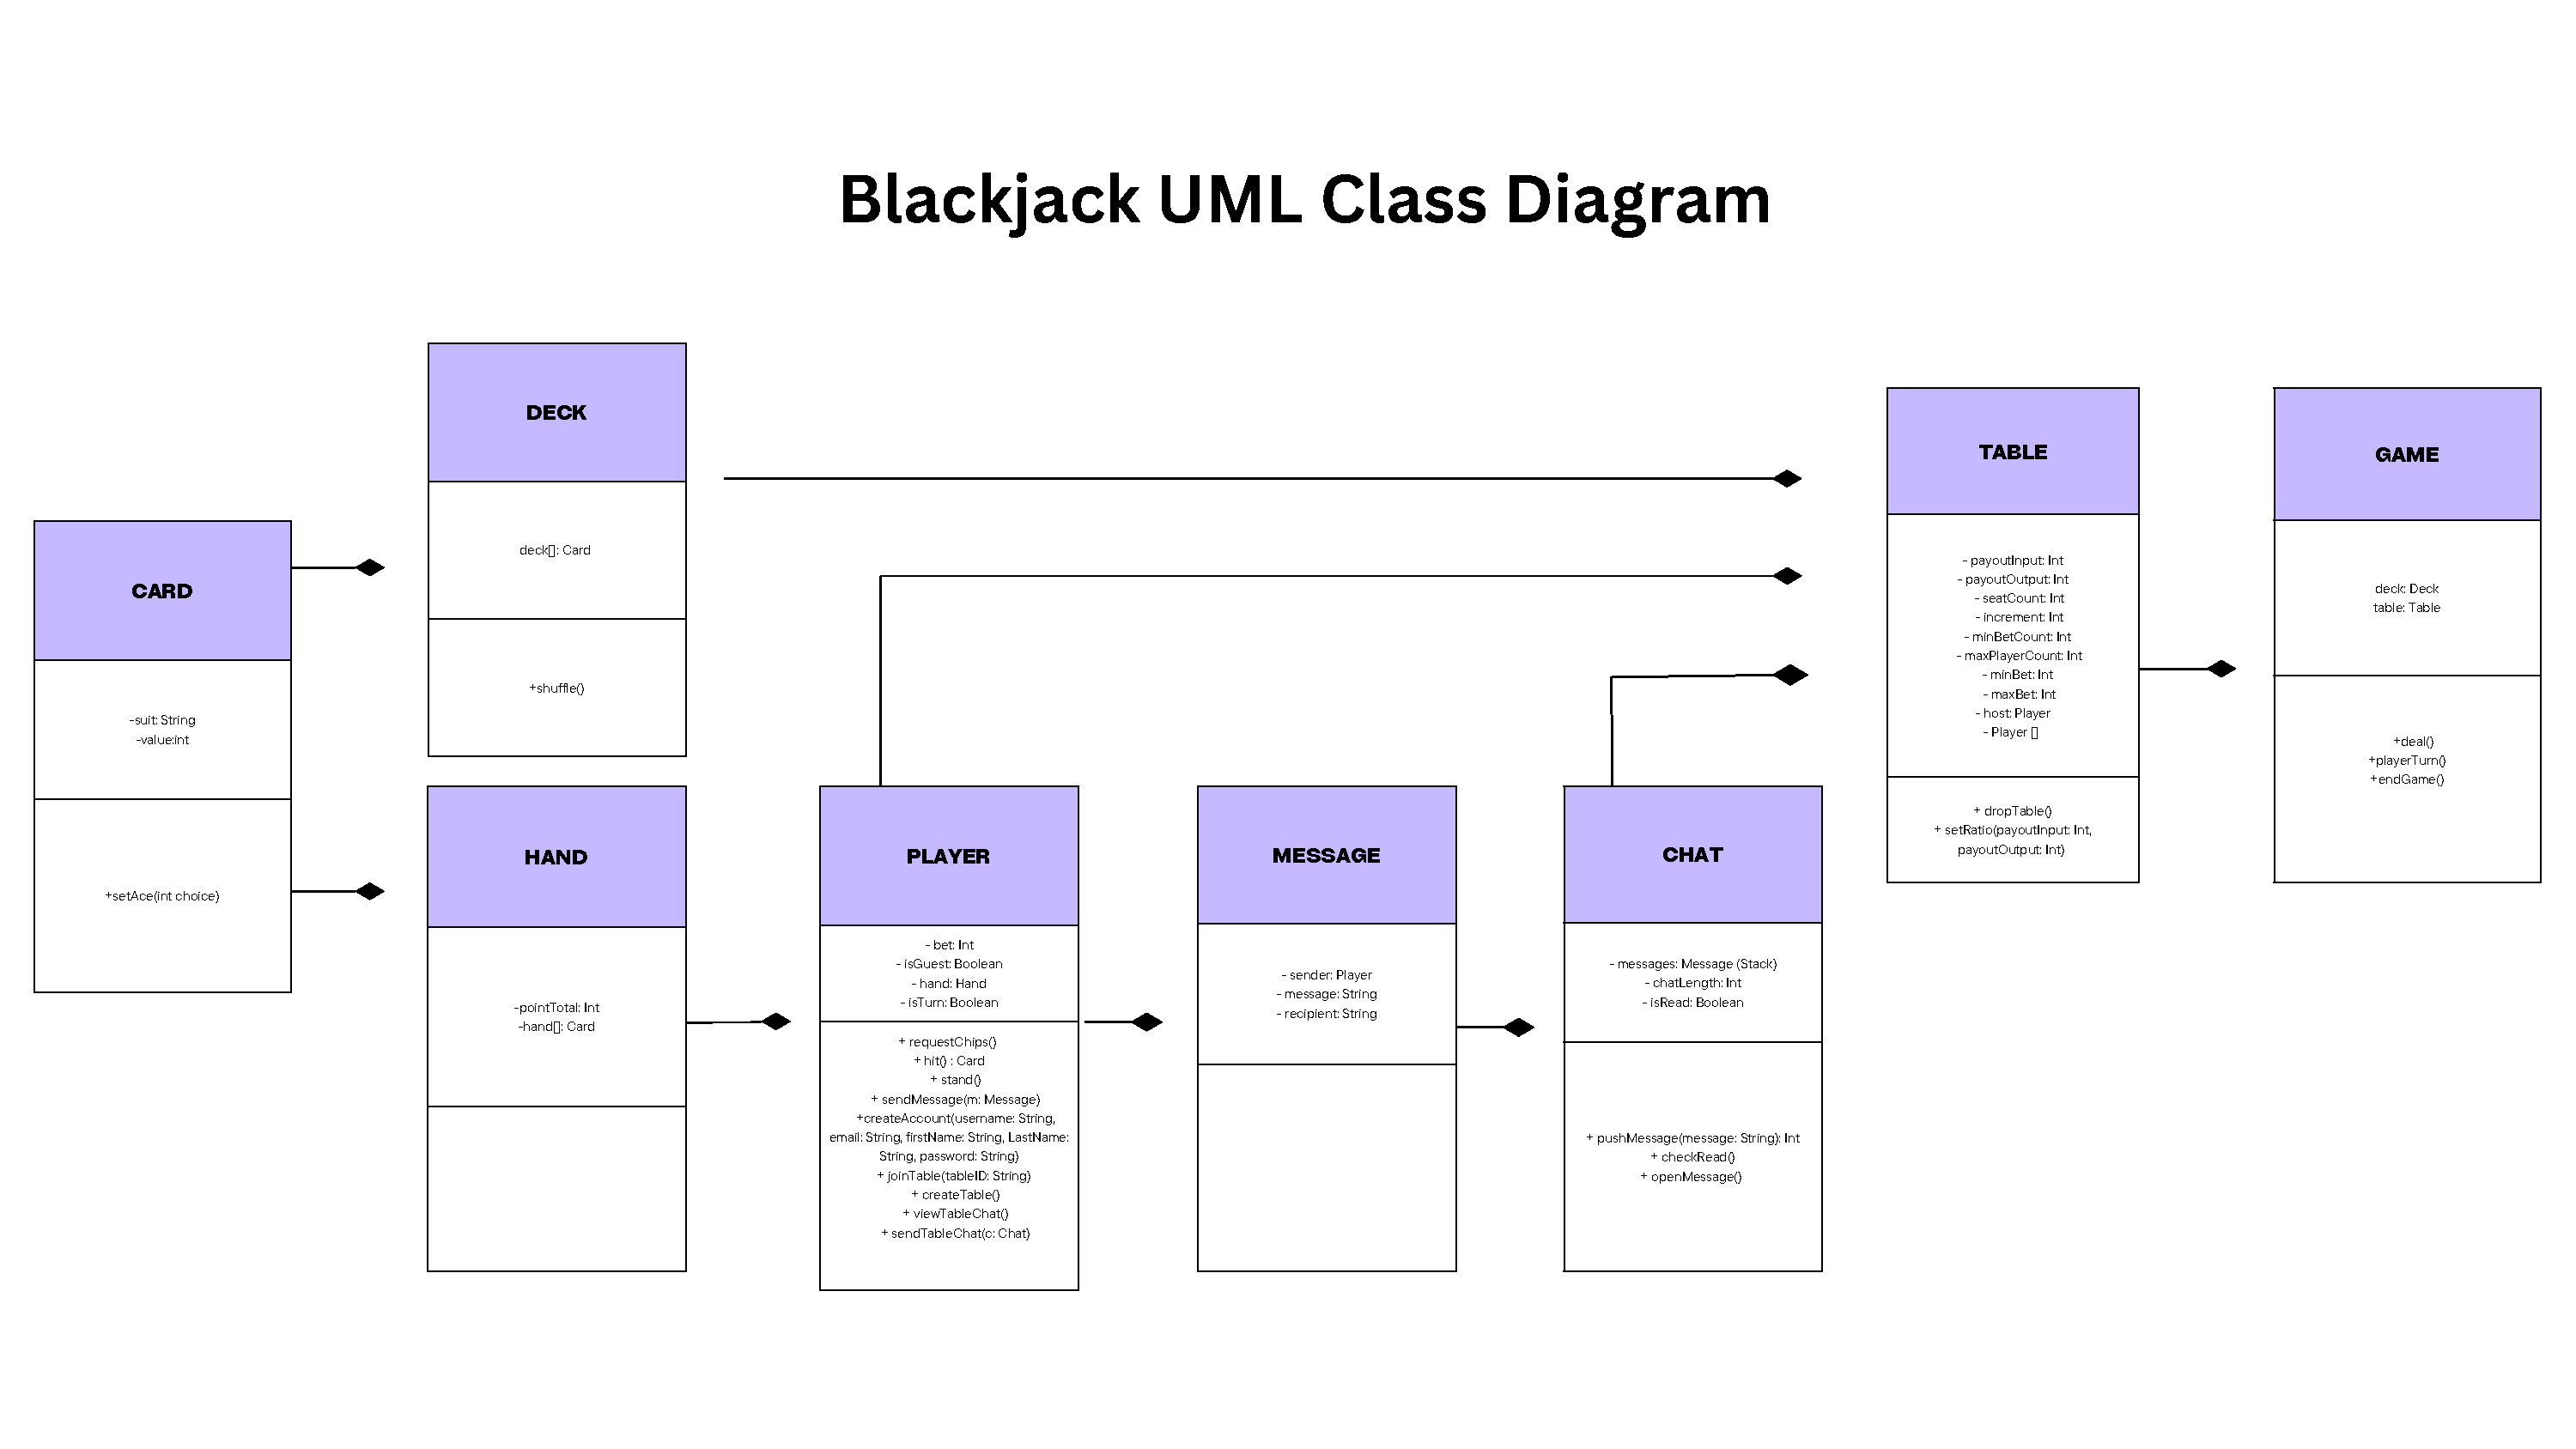
\includegraphics[width=0.8\linewidth]{figures/UML Diagram Whiteboard.pdf}
    \caption{UML diagram of major classes and relations.}
    \label{fig:UML}
\end{figure}

\pagebreak

\subsection{UI Mockups}
Here are some of the initial UI designs for our project:

\begin{figure}[hbt!]
    \centering
    
\includegraphics[width=0.5\textwidth]{figures/Blackjack.png} \\
    \caption{This is the UI mockup for the logo of the app (illus. Emma Heiser)}
    \label{fig:logo}
\end{figure}

\begin{figure}[hbt!]
    \centering
    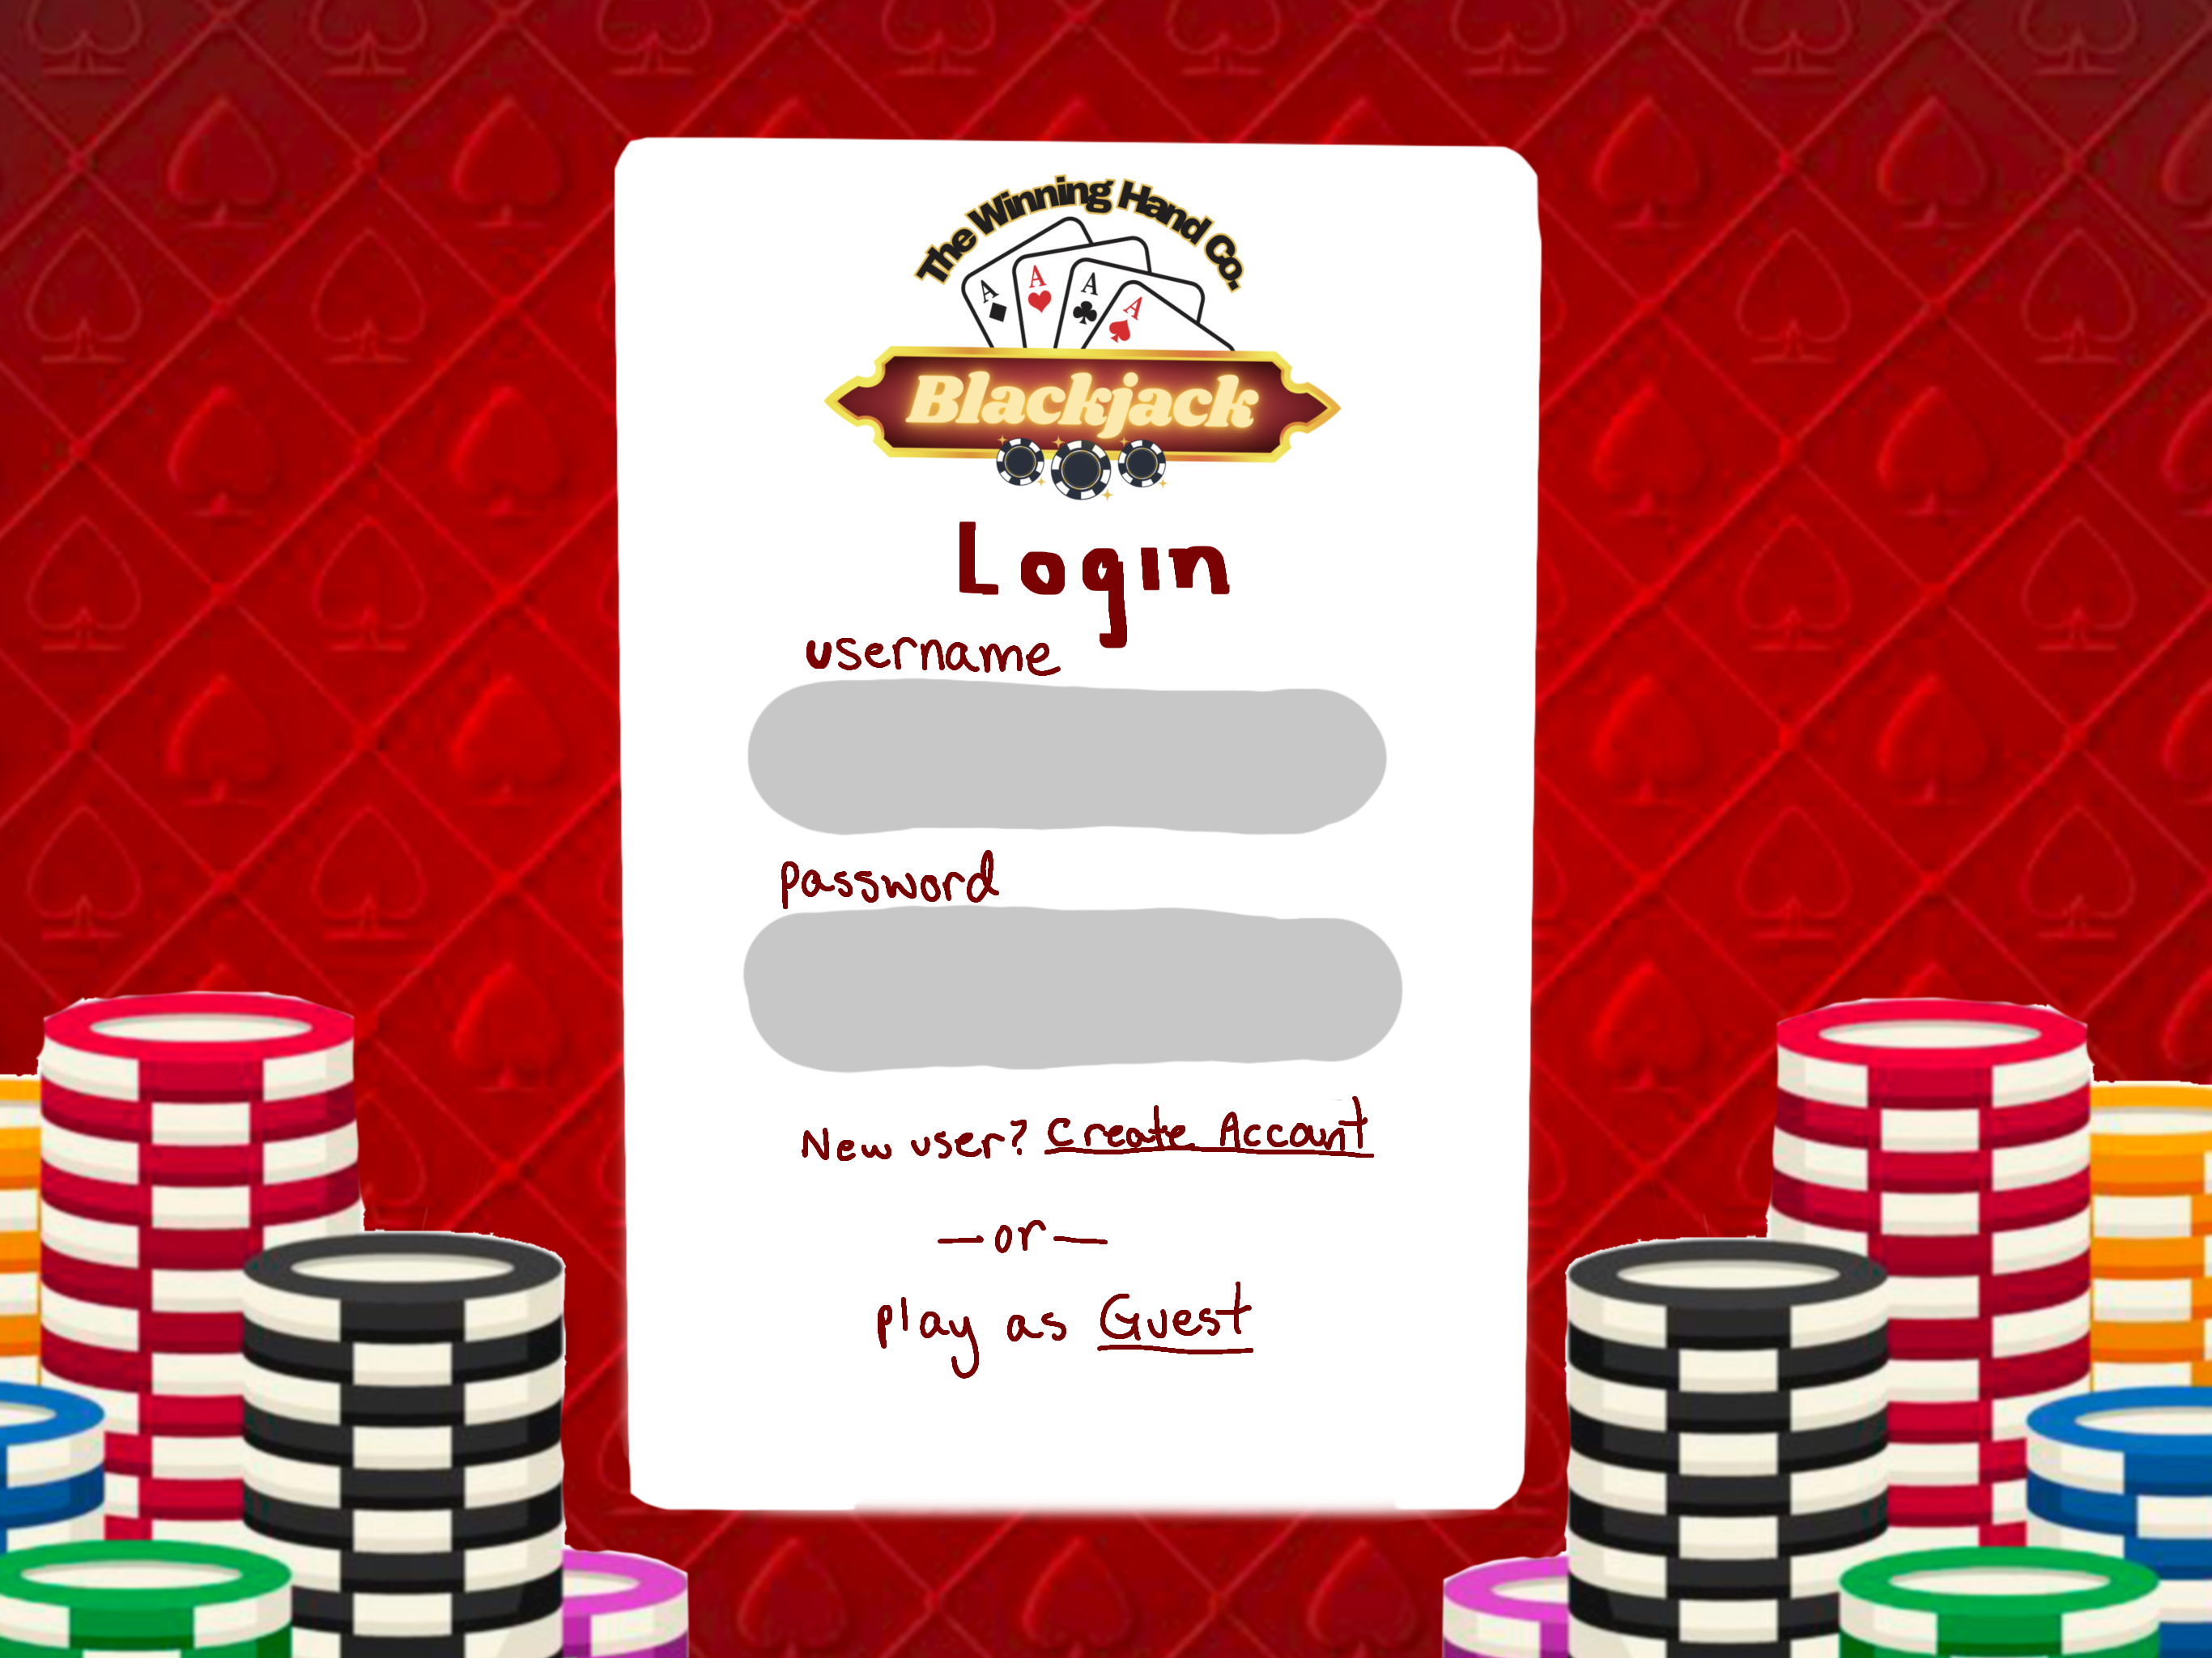
\includegraphics[width=0.75\linewidth]{figures/login.png}
    \caption{This is a UI mockup of the login screen (illus. Emma Heiser)}
    \label{fig:login}
\end{figure}

\begin{figure}[hbt!]
    \centering
    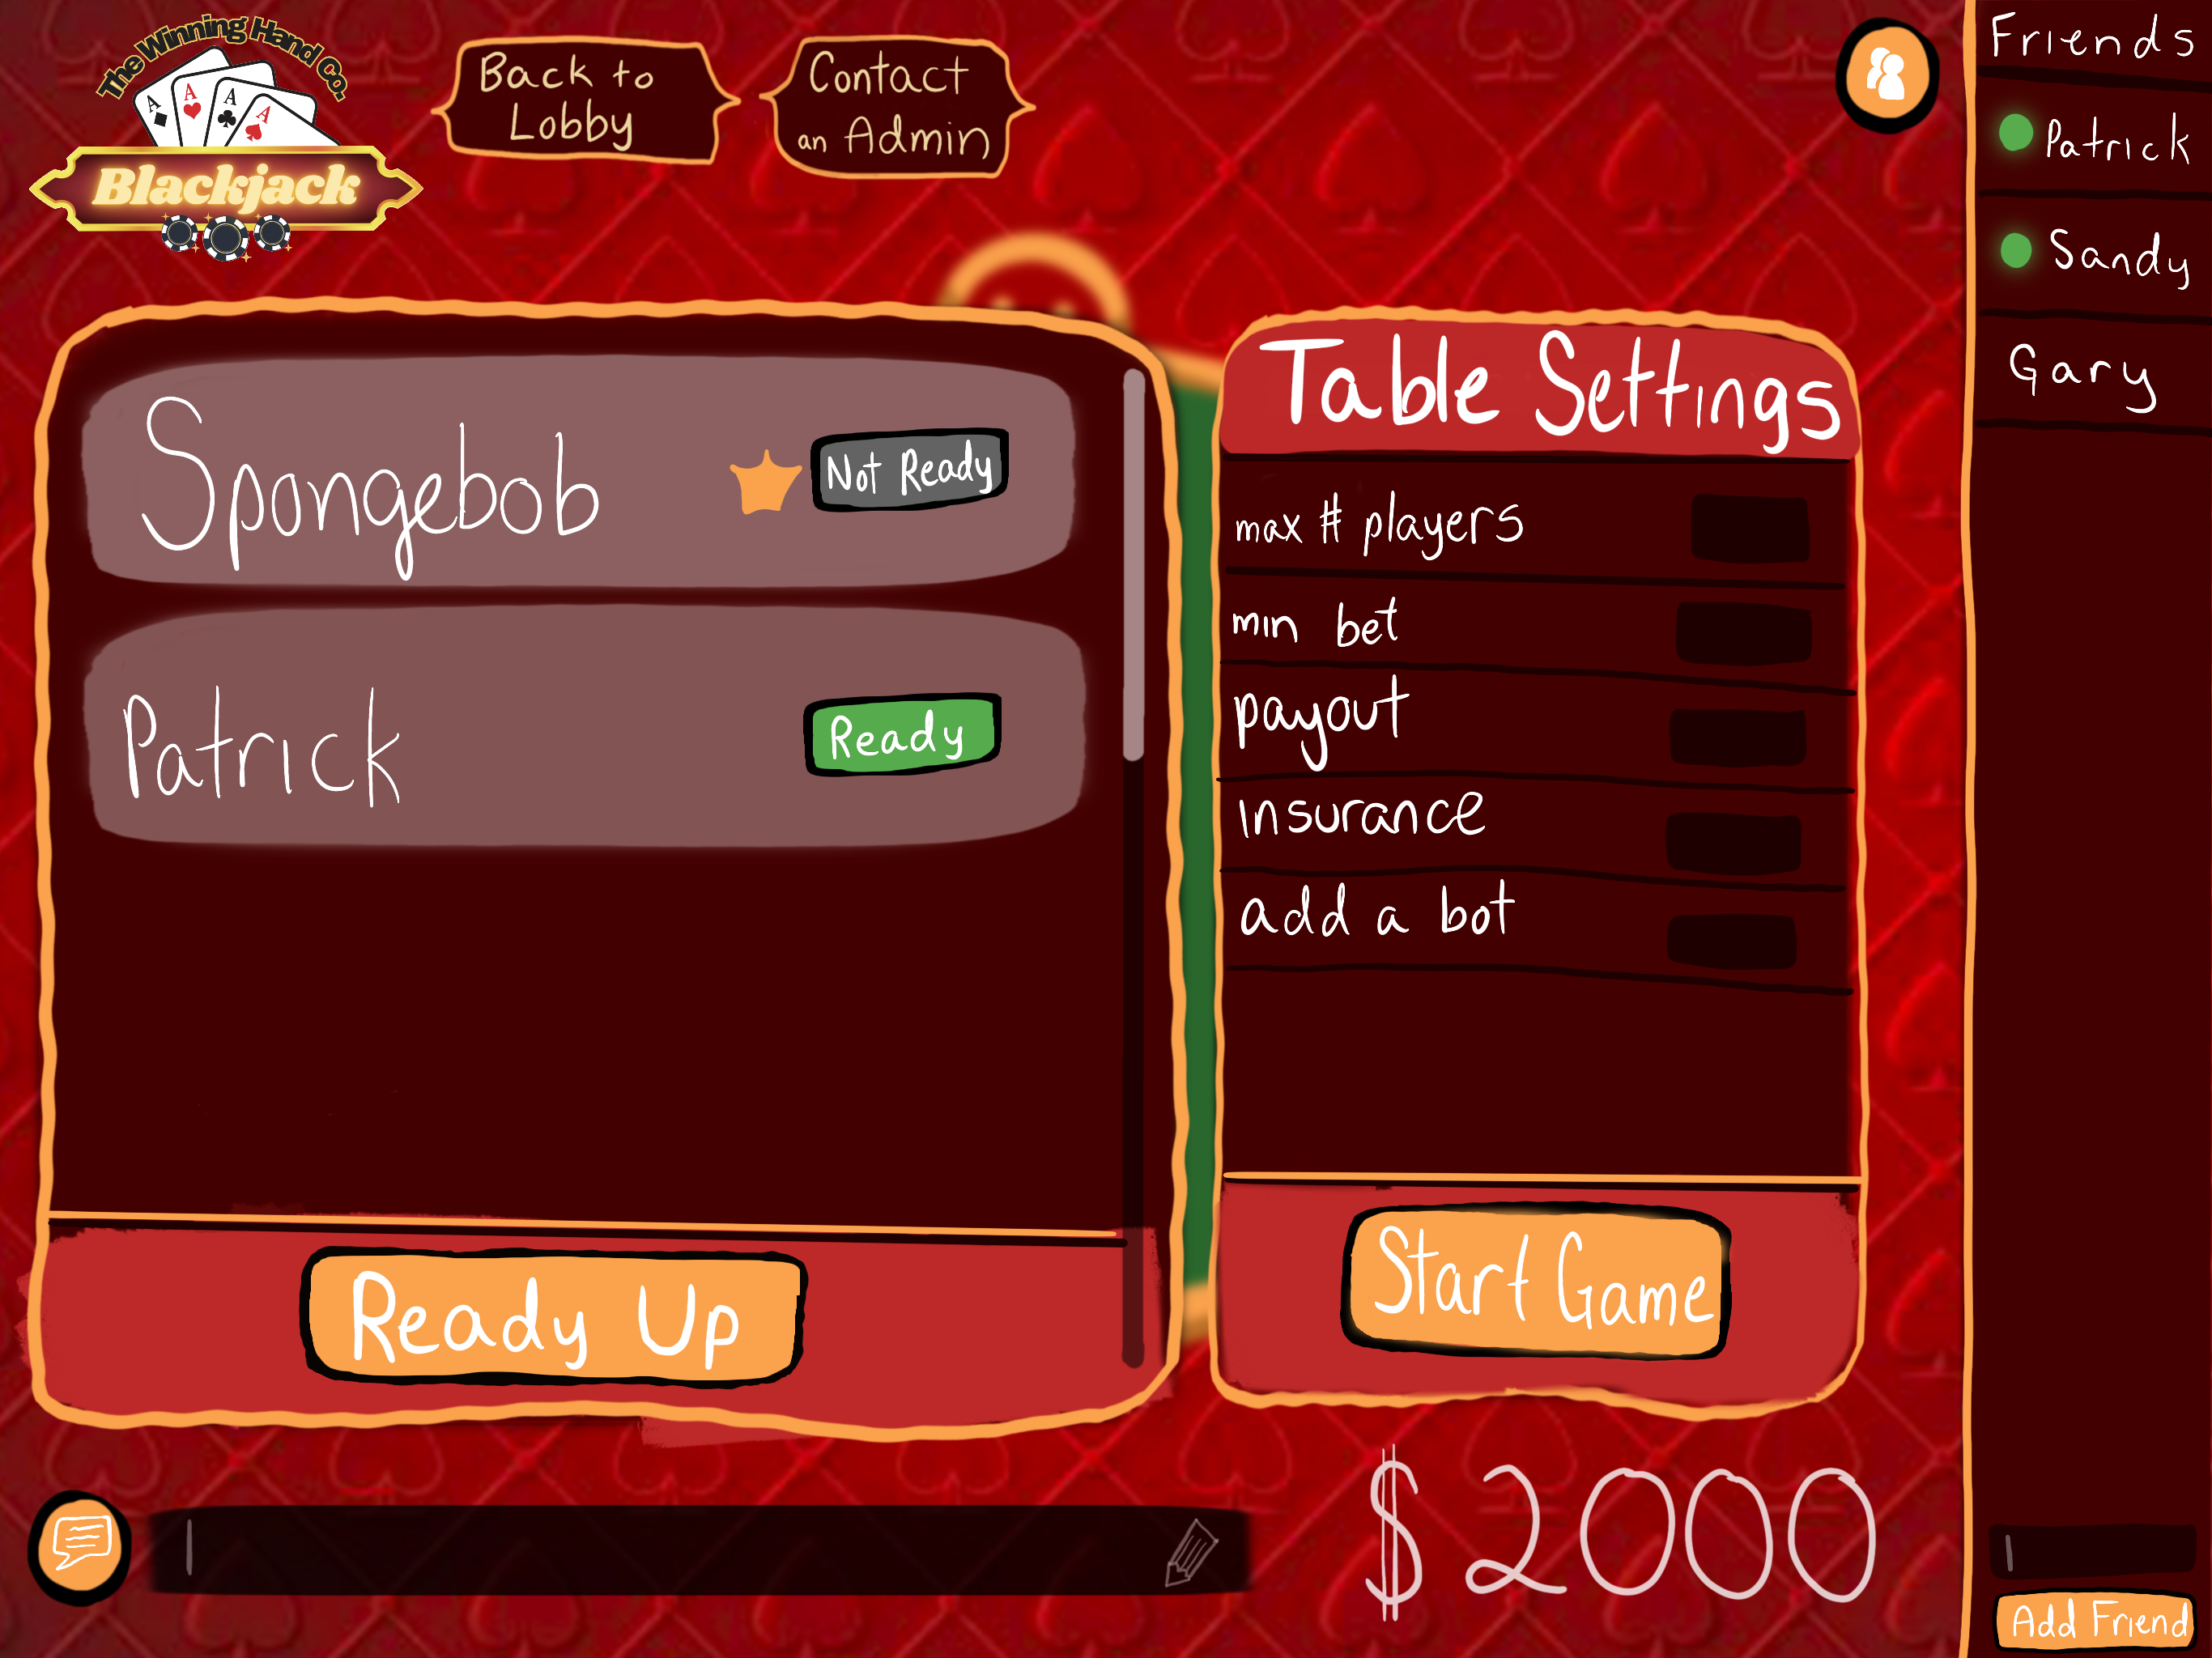
\includegraphics[width=0.75\linewidth]{figures/at-table.png}
    \caption{This is the UI mockup of creating a table (illus. Emma Heiser)}
    \label{fig:table}
\end{figure}

\pagebreak

\begin{figure}[hbt!]
    \centering
    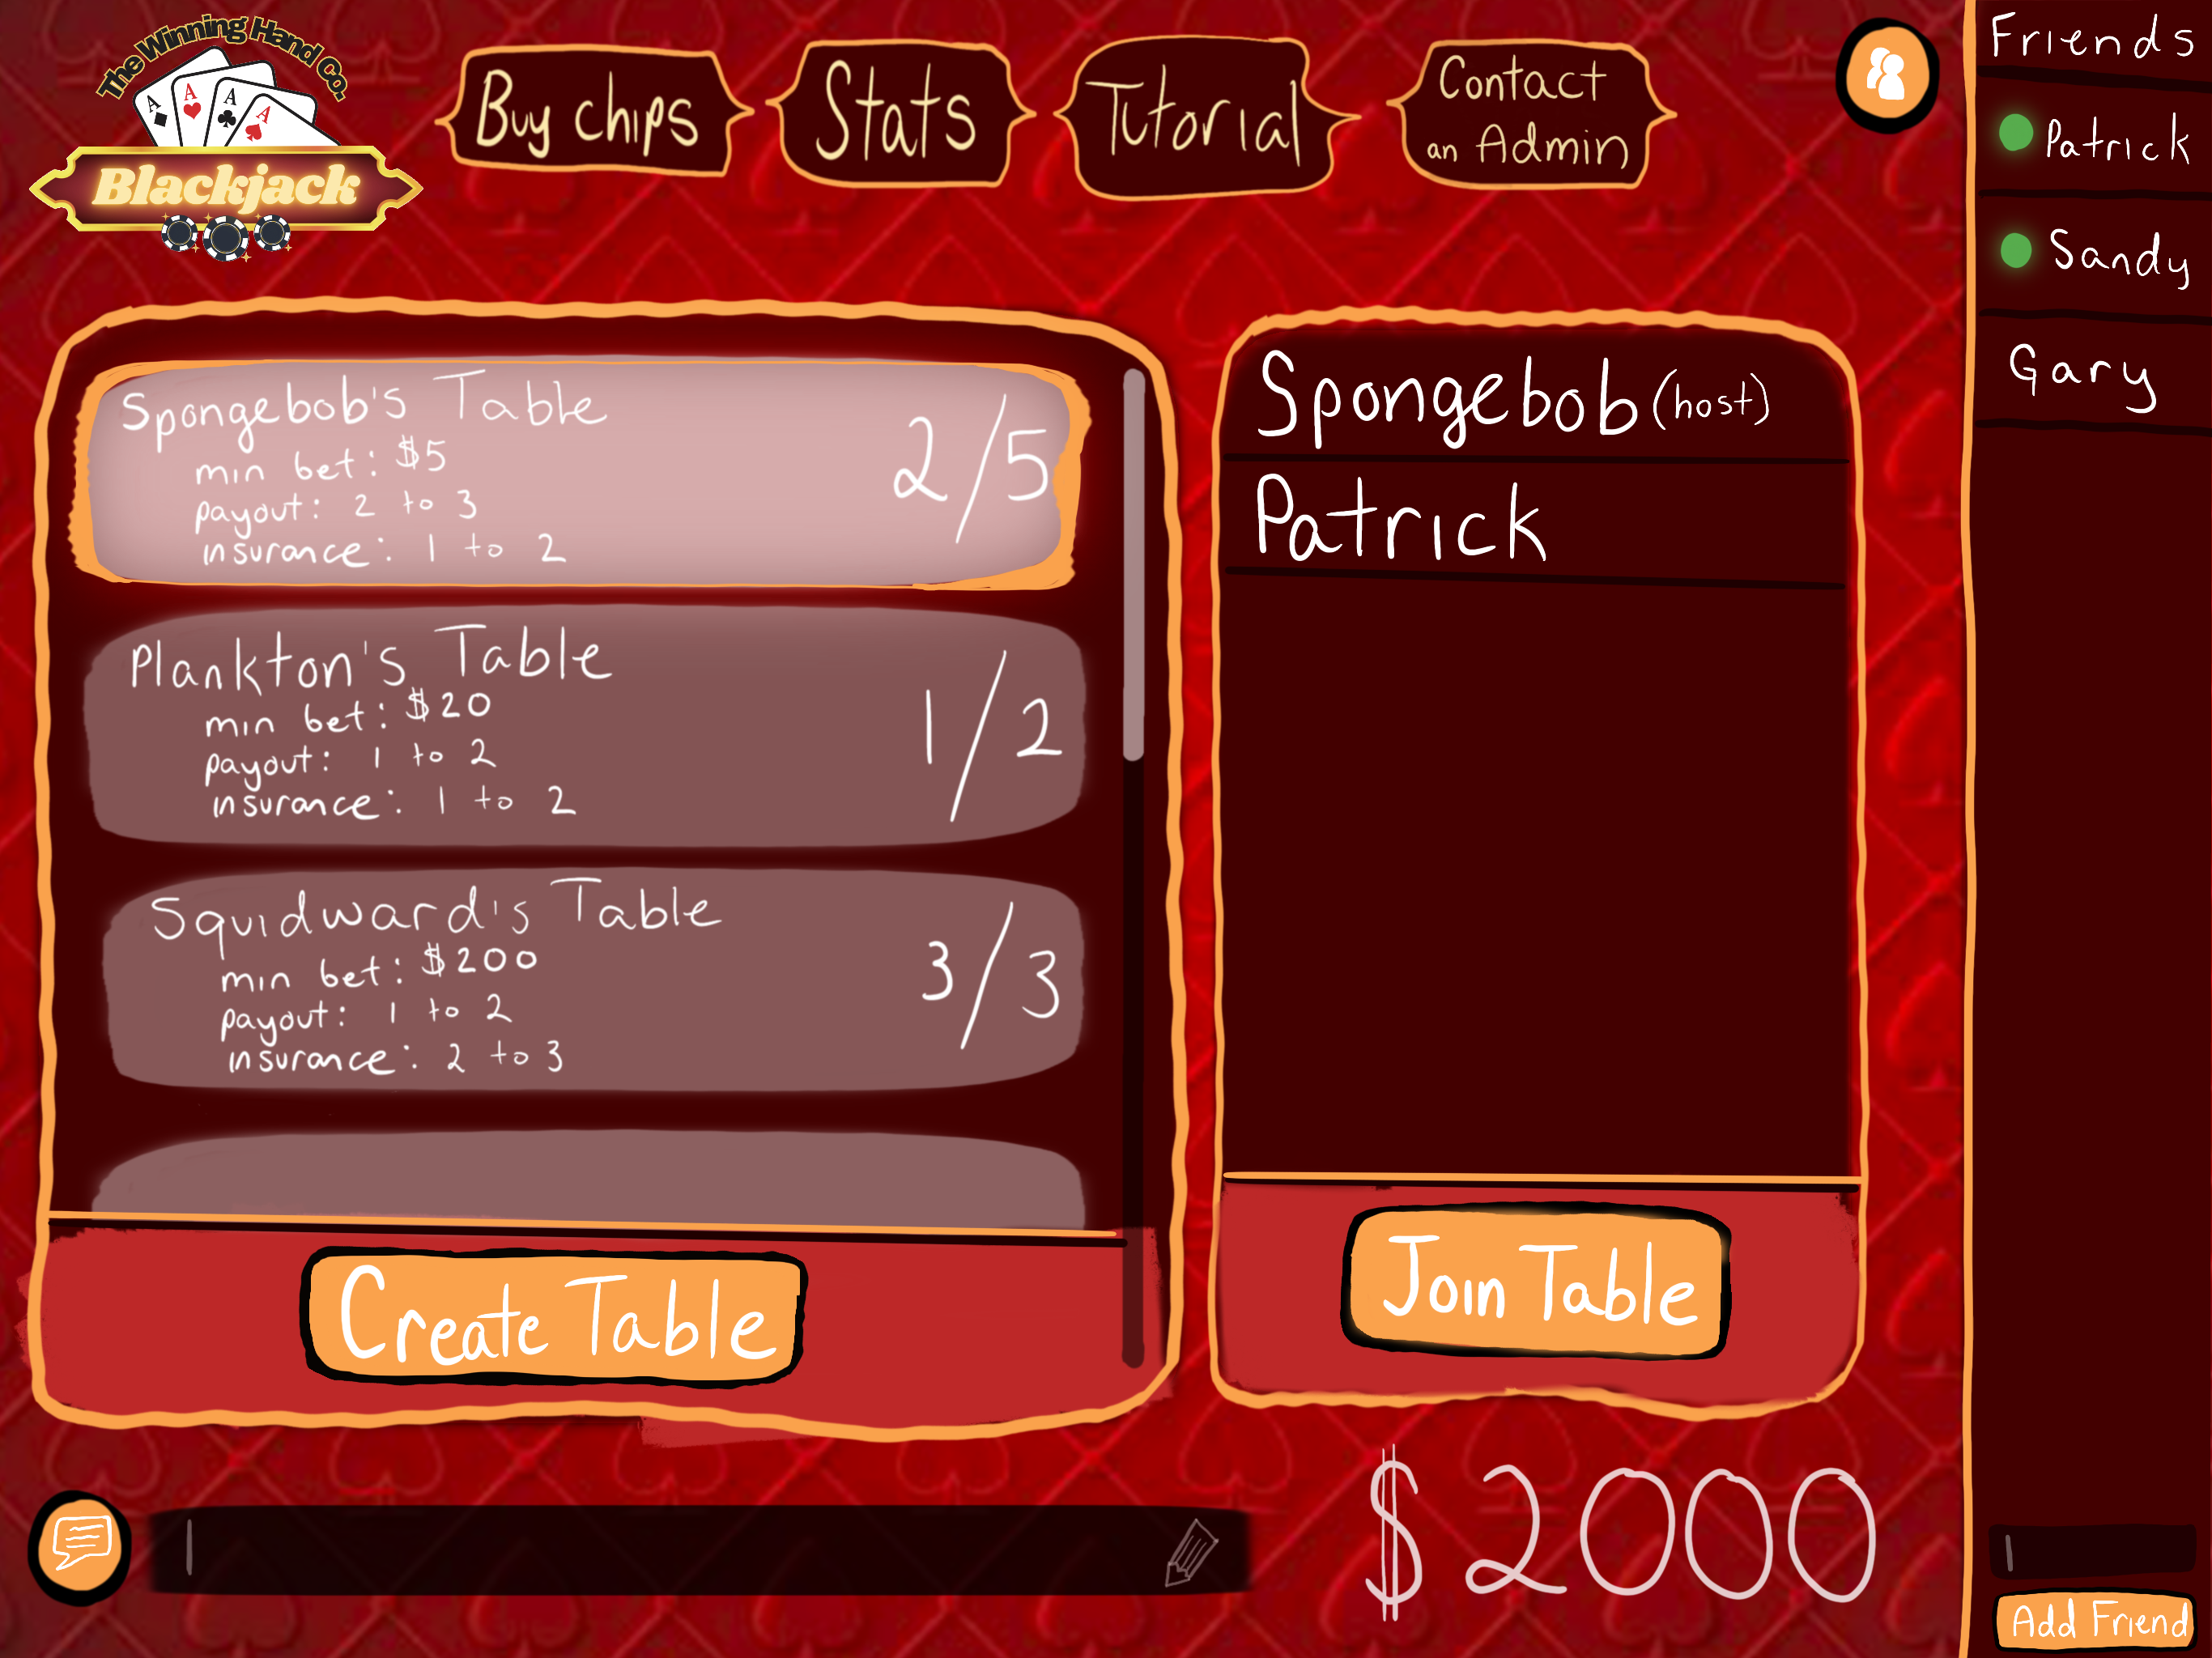
\includegraphics[width=0.75\linewidth]{figures/lobby.png}
    \caption{This is the UI mockup for the lobby where players can see available tables (illus. Emma Heiser)}
    \label{fig:lobby}
\end{figure}

\begin{figure}[hbt!]
    \centering
    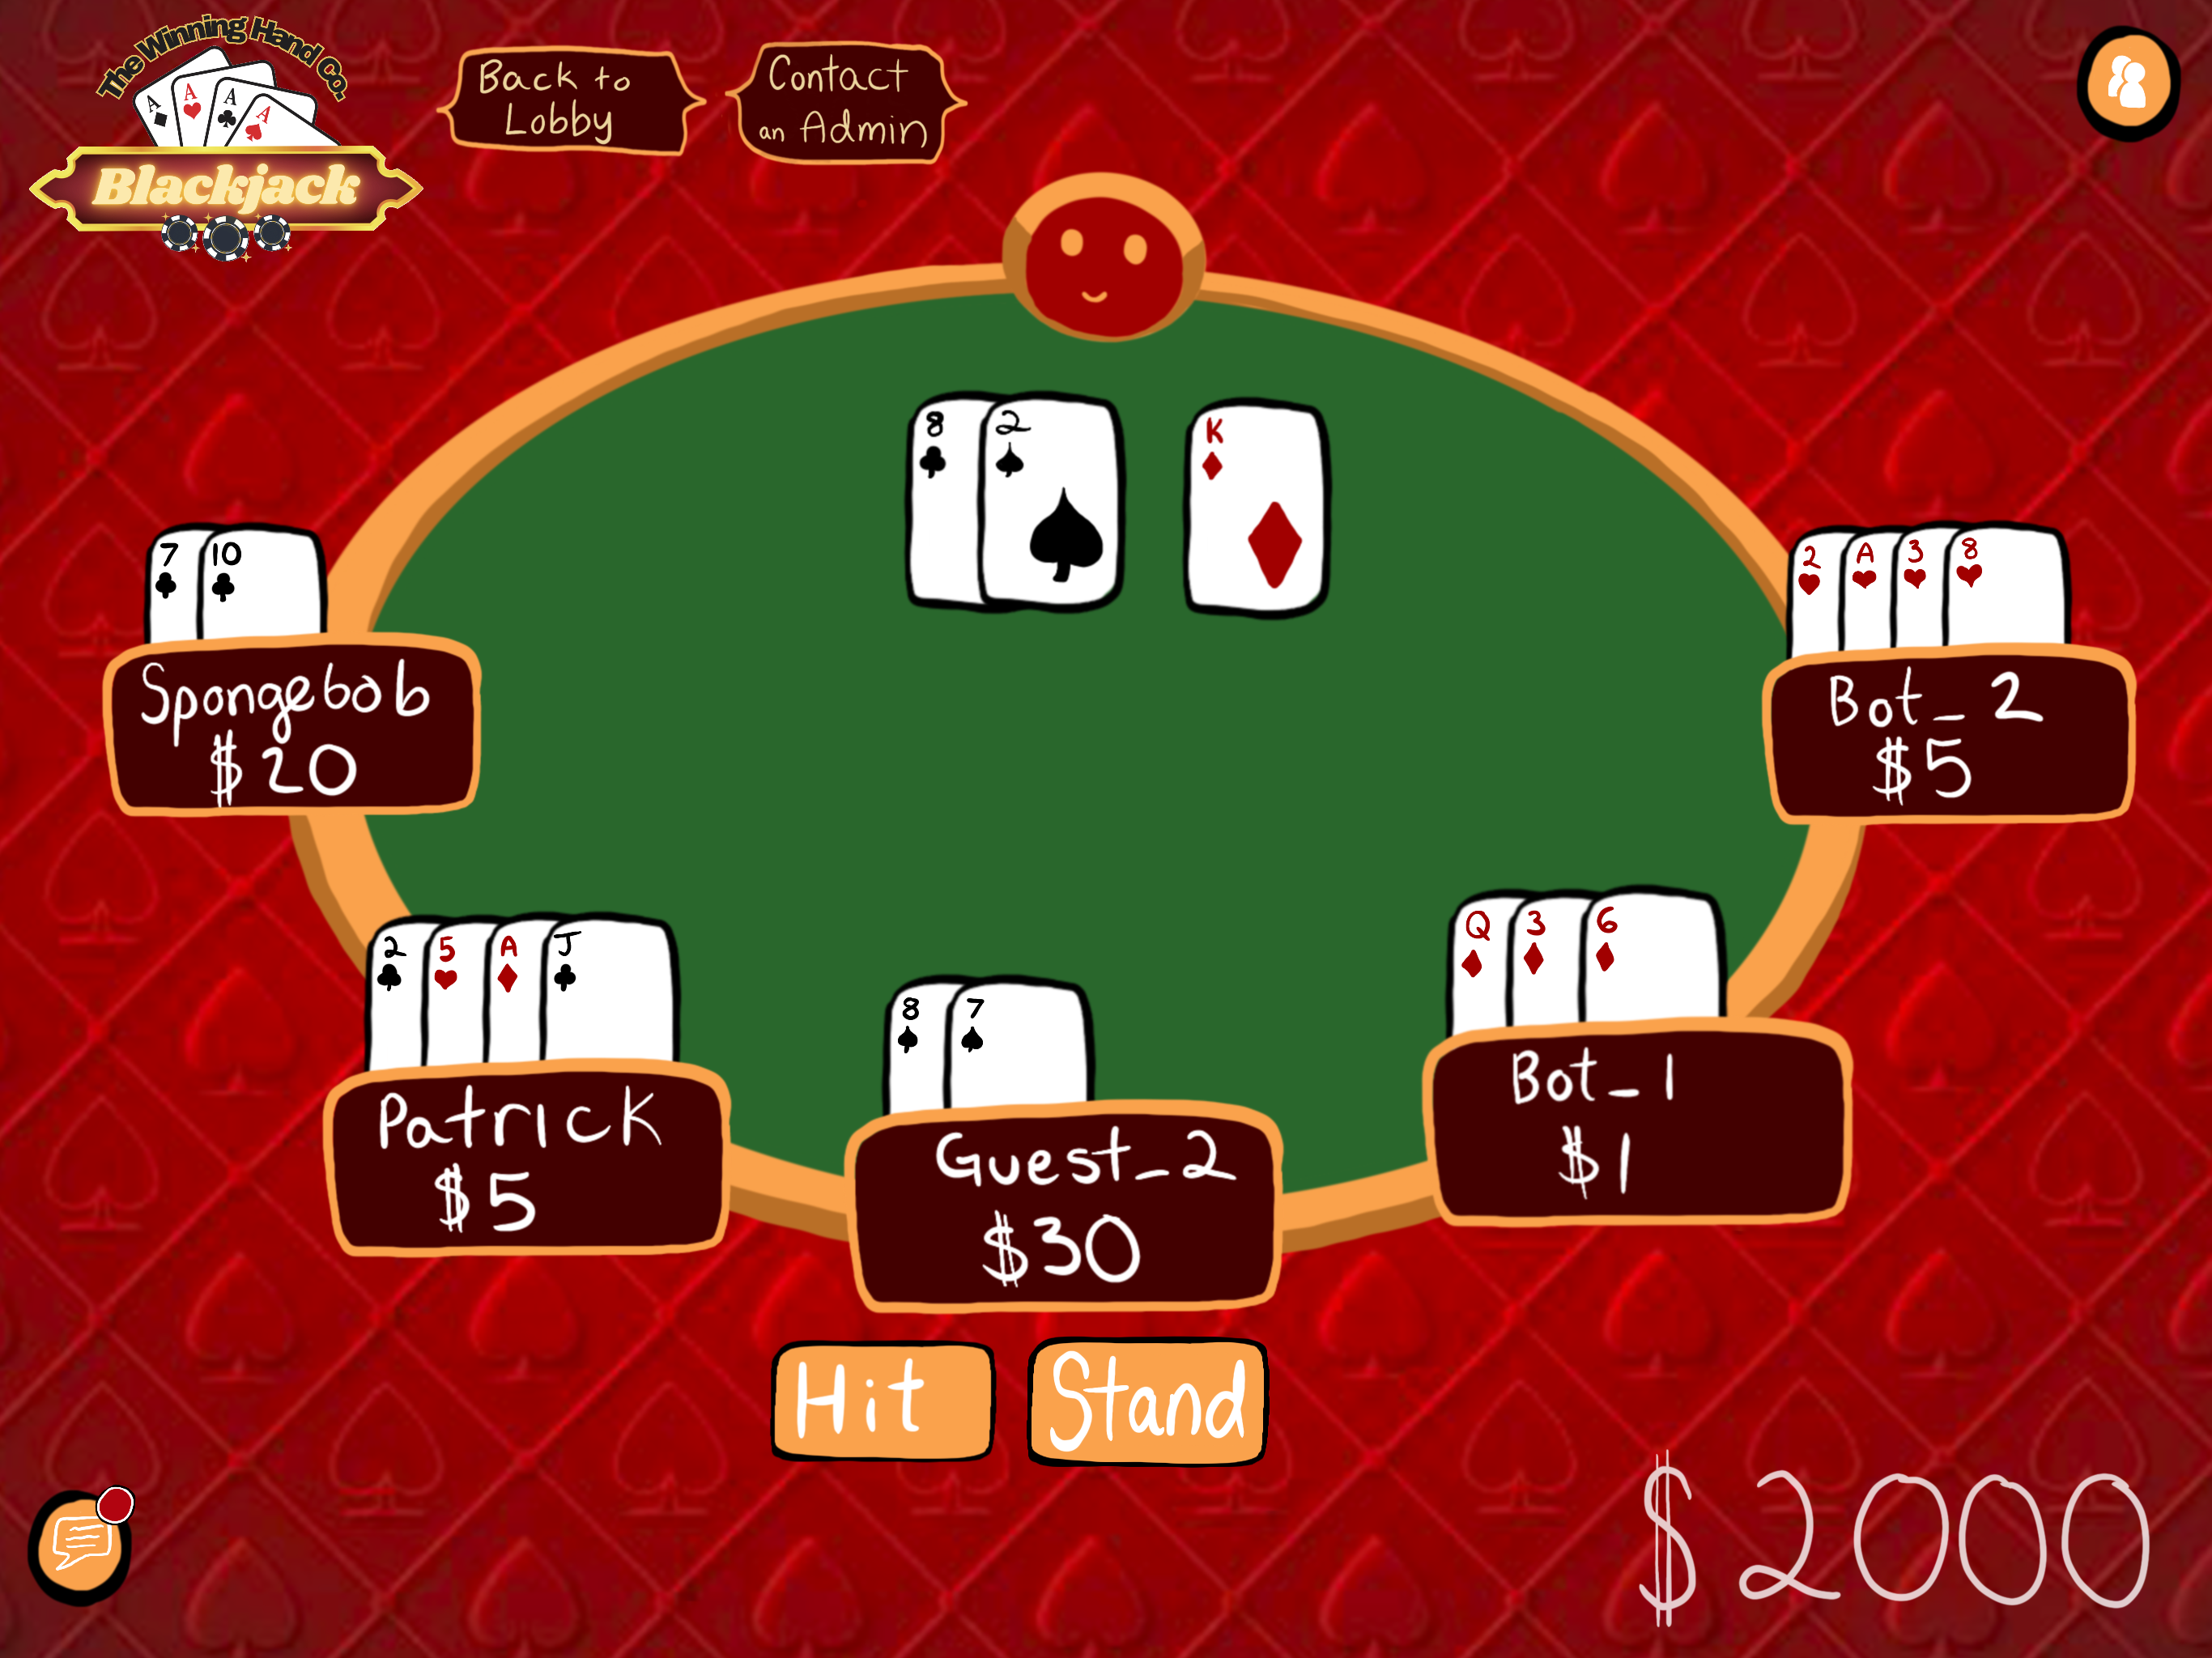
\includegraphics[width=0.75\linewidth]{figures/in-game.png}
    \caption{This is the UI mockup of the game being played at a table (illus. Emma Heiser)}
    \label{fig:game}
\end{figure}

\pagebreak

\section{Testing}
%[[ include test plan and coverage data

For our testing we will be using JUnit. We will be focused on writing good tests rather than achieving a set percentage required to commit. We believe that this is a reliable way to ensure that good software is being developed. However, if we \textit{had} to give a numerical value, we decided that 80\% coverage would be sufficient to commit.

\begin{figure}[!hbt]
    \centering
    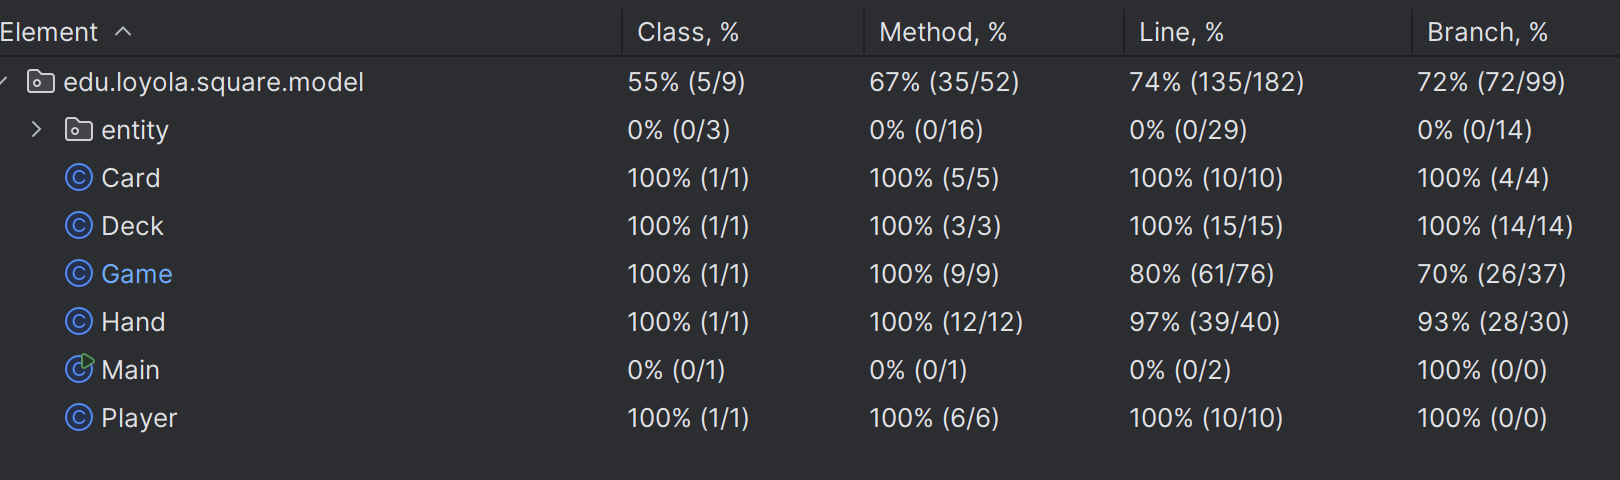
\includegraphics[width=1.0\linewidth]{figures/Coverage report (Model).png}
    \caption{Sprint 1 Coverage report (Note that the entity folder is being erroneously tested)}
    \label{Coverage report}
\end{figure}

%Briefly describe how you incorporated testing into each two week coding iteration. 
%What tool(s) proved useful? 
%What went well in terms of testing?
%What did not?

%]]
 
\section{Reflections on the Project \textbf{[TBD]}}



%\section{References}
\bibliographystyle{plain}
%\bibliography{references}


%\section{\LaTeX ``Tutorial''}

%OMIT this section in production, but here is some sample \LaTeX~to munch on.

%Use the table environment to include tables.
%Be sure to keep the label and caption below the tabular!

%Setting up tables can be annoying. You can also set it up in excel and then
%copy it into \textsf{https://www.tablesgenerator.com} to generate the latex. 

% Please add the following required packages to your document preamble:
%\usepackage[table,xcdraw]{xcolor}
% Beamer presentation requires \usepackage{colortbl} instead of 

% Please add the following required packages to your document preamble:
% \usepackage{graphicx}
% \usepackage[table,xcdraw]{xcolor}
% Beamer presentation requires \usepackage{colortbl} instead of \usepackage[table,xcdraw]{xcolor}

%\begin{table}[h!]
%    \centering
%    \begin{tabular}{|c|c|c|c|c|}
%    \hline
%      Risk   & Impact & Priority  & Overall Rating  & Mitigation \\
%         &  &  &  & \\\hline
%         &  &  &  & \\\hline
%         &  &  &  & \\\hline
%    \end{tabular}
%    \caption{Risks to the software.}
%    \label{tab:risks}
%\end{table}

%Table~\ref{tab:risks} overviews the risk relevant to our project.


%Use the figure environment to include images such as \textsf{.png} in your latex document. \\

%Figure~\ref{fig:class} shows the high-level class diagram.


%\begin{figure}[!bht]
%\begin{lstlisting}[language=Java]
%public static void main(String [] args)
%{
%  System.out.println("Hello World!");
%}
%\end{lstlisting}
%\caption{Hello Example.}
%\label{fig:hello}
%\end{figure}

%Figure~\ref{fig:hello} shows the code used to print hello.
%\textbf{Note that you writeup should include code sparingly.
%The details of the code are not its focus.}



\end{document}

